\documentclass[11pt]{article}
\usepackage[T1]{fontenc}
%^\usepackage[utf8]{inputenc}
\usepackage{amsmath,mathrsfs,bm}
\usepackage{color}
%\usepackage{cleveref}
\usepackage{mathtools}
\usepackage{graphicx}
\usepackage[font=scriptsize,labelfont=bf]{caption}
\usepackage{wrapfig}
\usepackage[compact]{titlesec}

\usepackage{natbib}
\usepackage[superscript,biblabel]{cite}

%\usepackage{fullpage}
\usepackage[margin=0.5in]{geometry}

\pagenumbering{gobble}

\usepackage{fontspec}
\setmainfont{Arial}

% \linespread{1.05}
\newcommand{\jb}[1]{{\color{blue} (#1)} }
\newcommand{\gs}[1]{{\color{red} #1}}

\setlength{\parskip}{0pt}

\makeatletter
\renewcommand{\paragraph}{%
  \@startsection{paragraph}{4}%
  {\z@}{1ex \@plus 1ex \@minus .2ex}{-1em}%
  {\normalfont\normalsize\bfseries}%
}
\makeatother

\begin{document}




\subsection*{Significance and Background}

% A large proportion of common diseases (i.e. prevalence > \jb{XX}\%) are genetically complex. In contrast to Mendelian diseases, genetic causation of complex diseases is not straightforward, with genetic risk for any given disease spread across a large number of genes, each individually of relatively minor effect. While successful efforts to map the genetics of Mendelian diseases date well back into the $20^{th}$ century, only in the past decade with the maturation of the genome wide association study (GWAS) approach has some understanding of the genetic basis of complex disease begun to emerge\cite{Visscher:2012je,get_more}. It's become clear now that estimates of heritability based on the twin study design were broadly accurate (if slightly overestimated in some cases), and that the heritabilities of common complex diseases are generally high. GWAS and related approaches have also shown that a substantial proportion of the variance in risk can be attributed to a very large number of common alleles \cite{Consortium:2009ef, Lee:2012iu,Loh:2015hz, Ripke:2014eb}, while sequencing and exome studies indicate a role for rare variants of large effect as well \cite{Richards:2016cs, Genovese:2016fv, Purcell:2014gw}. The totality of the evidence therefore suggests that thousands or perhaps even tens of thousands of individual genetic variants play a role in determining susceptibility to any given complex disease. Less clear however is our understanding of the forces which govern the prevalence and genetic architecture (i.e. the relationship between allele frequency and effect size) of complex disease. In contrast to Mendelian diseases, where nearly a century of theory explain how mutation rate, dominance, selection \cite{Patil:2010ha} and demography \cite{HurlesText} combine to influence the prevalence of these diseases, there is relatively little in the way of quantitative theory on the evolution of complex disease. 


Most common diseases (those with prevalence > 0.1\%, including for example schizophrenia, autism, and diabetes to name a few) are complex. In contrast to Mendelian diseases, the risk of developing complex diseases is affected by variants at many loci across the genome, each of which typically has low penetrance. While the genetic basis of many Mendelian diseases have been successfully mapped during the $20^{th}$ century, the systematic mapping of variants underlying complex diseases became possible only over the last decade with the maturation of the genome wide association study approach.\cite{Risch:1996ub,Visscher:2012je,get_more} GWAS and related variance partitioning methods have largely validated estimates of heritability based on the twin studies (although, in some cases the latter were slight overestimates), and thus shown that the heritabilities of common complex diseases are generally high. They have also shown that the bulk of the variance in risk can be attributed to a very large number of common
alleles (generally each with small effects),\cite{Consortium:2009ef,Lee:2012iu,Loh:2015hz,Ripke:2014eb,Lee:2012iu} while sequencing and exome studies indicate a potential role for rare variants with larger effect as well.\cite{Richards:2016cs, Genovese:2016fv, Purcell:2014gw} While the significant associations for even the most successful disease GWAS number in the hundreds, statistical analyses of GWAS results indicate that many thousands of variants affect their susceptibility \jb{refs}.

However, we still remain unclear about why complex diseases are as common as they are, and what determines their genetic architecture, i.e. the observed relationships between variants’ effect size and frequency. In contrast to Mendelian diseases, where we have a fairly good quantitative understanding of how the mutational target size, recessivity, selection and demography combine to determine disease prevalence and allele frequencies, we lack a satisfactory quantitative framework describing how these factors and others determine the prevalence and architecture of complex diseases. 



% \jb{need to introduce idea of variation in prevalence and architecture as tool to greater understanding}
% Variation in the prevalence of diseases with similar fitness costs may then simply be down to difference in their mutational target sizes, and variation in genetic architectures may arise chiefly from differences in the distribution of mutational effect sizes. Conversely, variation in the fitness costs of specific diseases will lead to differences in the strength of direct selection against risk incresing variants associated with those diseases, which should account for some amount of variation in both architecture and prevalence.


We do have, nonetheless, a qualitative understanding of some of the population genetics process that affect genetic variation for complex diseases. Perhaps most straightforward is that genetic variation for disease risk reflects a balance between mutation and selection.\cite{Johnson:2005do} This suggests that a given genetic disease is common if it has a large mutational target sizes; that variation in prevalence among diseases with similar fitness costs reflects differences in target sizes; and that variation in genetic architectures arises from differences in the distribution of mutational effect sizes. Similarly, differences in the fitness costs among diseases should lead to differences in the strength of selection on variants (that have similar effects on disease risk), which would also cause variation in both architecture and prevalence. 

However, selection acting on mutations due to their effect on a given disease is only part of the story, as ample evidence suggests that variants affecting a given disease often have pleiotropic effects on other traits that are themselves under selection\cite{Pickrell:2016ko, Visscher:2016fp}. The genetic architecture of a given disease may then reflect both direct selection due to the disease as well as indirect selection due to these pleiotropic relationshipsto other diseases or quantitatie traits\cite{Fraser:2013jj,Berg:2014bs, Corona:2013cl, Chen:2012jv, Ayub:2014hk,Polimanti:2017bv}. The effects of pleiotropy on disease prevalence and architecture are far from straightforward and await a more systematic treatment (see below).

% For example, mutations that increase the risk of a given disease may have protective effects on other diseases\cite{Fraser:2013jj,Berg:2014bs, Corona:2013cl, Chen:2012jv, Ayub:2014hk,Polimanti:2017bv}, and more generally may affect other traits, thus complicating the relationship between a mutations effect size on the disease under consideration and its effect on fitness. The effects of pleiotropy on disease prevalence and architecture are far from straightforward and await a more systematic treatment (see below).  

Lastly, recent changes to the environment have also likely affected the prevalence and architecture of complex diseases. For example, the “thrifty gene” hypothesis\cite{Neel:1962tj, Neel:1999tu} posits that diseases such as type 2 diabetes and hypertension exhibited a drastic increase in prevalence due to profound recent changes in diet and lifestyle, which caused a mismatch between the ancestral human environment and present conditions. A recent study documenting rapid changes in the prevalence of type 2 diabetes and obesity in response to food shortage and economic crisis in Cuba in the 1990s\cite{Franco:2013hb}, illustrates this effect. It has been further suggested that such profound changes may disrupt developmental canalization, leading to wholesale changes to the distribution of genetic effects on disease risk\cite{Gibson:2000vi, Gibson:2009ie}. While some of these ideas likely apply to some diseases (and they are also not mutually exclusive), they generally lack quantitative predictions that allow for them to be rigorously tested and for their effects to be quantified. 




% Nonetheless, several qualitative mechanisms have been proposed which may potentially explain the observed patterns. Perhaps the most straightforward is that the present distribution of genetic risk reflects a simple balance between mutation and selection \cite{Johnson:2005do}. The prevalence of common disease may therefore be ascribed to relatively large mutational target sizes for many diseases. Variation among diseases in their prevalence and genetic architectures may simply reflect difference in features such as the mutational target size, distribution of effects, and fitness cost of the disease. The direct selection experienced by a given allele is likely only part of the story, however, as the extreme polygenicity of complex diseases indicate that pleiotropy must almost surely be extensive \cite{Pickrell:2016ko, Visscher:2016fp}. Indirect selection due to these pleiotropic effects may therefore play a major role in determining architecture and prevalence, both in steady-state scenarios, where pleiotropic effects may alter the stregth of selection for or against disease alleles or under more dynamic hypotheses, where recent positive selection on a trait genetically correlated to disease may have altered prevalence and/or architecture, as has been argued in a number of cases with conflicting evidence \cite{Fraser:2013jj,Berg:2014bs, Corona:2013cl, Chen:2012jv, Ayub:2014hk,Polimanti:2017bv}. Alternative explanations invoke the recent and profound changes in the human environment (diet, lifestyle, etc.) and the possibility that the mismatch between the ancestral human environment and present conditions that have resulted in a large increase in disease prevalence \cite{Gibson:2000vi, Gibson:2009ie}. Such was the original basis for the ``thrifty genotype'' hypothesis \cite{Neel:1962tj, Neel:1999tu}, and subsequent observation of large scale oscilations in type 2 diabetes incidence in response to food shortage and economic crisis and subsequent recovery in Cuba in the 1990s \cite{Franco:2013hb} indicate that this effect can be profound indeed. While some of these ideas likely apply to some diseases (and they are also not mutually exclusive), more often than not they have been put forward as verbal models only, and so it is difficult to quantitatively check their predictions.

Indeed, there has been surprisingly little work aimed at relating population genetic processes with the results emerging from GWAS. In this vein, two studies been especially influential. Pritchard\cite{Pritchard:2001hw} considered a model in which a mutation’s effect on disease risk is completely uncoupled from its fitness cost, i.e. an extreme pleiotropic limit. While this paper played a central role in grounding the debate surrounding the common disease-common variant hypothesis in population genetic theory\cite{Pritchard:2002ux}, many complex diseases are known to affect fitness \jb{refs} and the magnitude of variants’ effects on different traits are often correlated\cite{BulikSullivan:2015jf,Pickrell:2016ko,Visscher:2016fp}, suggesting that it is unrealistic to assume that a mutation’s effect on disease risk is independent of its effect on fitness. A second influential study by Eyre-Walker\cite{EyreWalker:2010dn} posited that all mutations are deleterious, but allows for their effect size, $\alpha$, and selection coefficient, $S$, to be related by the functional form: $\alpha = \delta S^{\tau} (1+\epsilon)$, where $\delta$ is a randomly chosen sign (i.e. $1$ or $-1$), $\epsilon$ is a normally distributed noise term, and $\tau$ is a “coupling parameter” meant to capture the effect of pleiotropy. When $\tau$ equals 1 a mutation's selection coefficient is tightly coupled to its effect on disease, and when it equals zero the model converges to Pritchard’s pleiotropic limit.\cite{Pritchard:2001hw} Eyre-Walker’s model has also been used as a basis for inferences based on GWAS results for type 2 diabetes\cite{Agarwala:2013bu,Fuchsberger:2016df} and prostate cancer\cite{Mancuso:2015cp} (see Aim 2 below for more background on the Eyre-Walker model in this context). However, the relationship between effect size and fitness in this model has little justification beyond mathematical convenience (and fact possesses some odd features, such as fitenss equivalence of mutations with opposing effects on disease). Moreover, more recent work illustrates that assuming a different relationship profoundly affects the predictions about genetic architecture\cite{Caballero:2015ce}. This suggests that understanding the relationship between GWAS findings and population genetics processes will require a more principled way of relating the effects of mutations on disease phenotypes with their effect on fitness.

% Each of these hypotheses are ultimately statements about population and quantitative genetic processes. While some models relating population genetic processes with the kind of data emerging from GWAS have been proposed, they generally rely on various \textit{ad hoc} or limiting assumptions that make easily interpretable inference difficult. Nonetheless, two studies in particular have been especially influential. Pritchard, in 2001\cite{Pritchard:2001hw}, considered a model in which the effect on disease risk is completely uncoupled from their fitness cost, i.e. an extreme pleiotropy limit. While this paper was enormously influential in grounding the debate surrounding the common disease-common variant hypothesis in population genetic theory\cite{Pritchard:2002ux}, it seems unrealistic that a mutation's effect on disease risk should not have any consequences for its fitness. A second study which has been influential is that of Eyre-Walker in 2010 \cite{EyreWalker:2010dn}, who posited that all mutations are deleterious \textit{a priori}, but arbitrarily assumed a relationship between effect size and selection coefficient of the form $\alpha =\delta S^\tau (1+\epsilon)$, where $S$ is the selection coefficient, $\delta$ is a randomly chosen sign (i.e. $1$ or $-1$), $\epsilon$ is a noise term, and $\tau$ is a ``coupling parameter'' meant to capture the effect of pleiotropy: where $\tau =1$ means no pleiotropy and $\tau=0$ gives Pritchard's \cite{Pritchard:2001hw} extreme pleiotropy limit. While this model has seen empirical application (see Specific Aim 2 below for more background on the Eyre-Walker model in this context), it does not have any obvious theoretical justification, and indeed possesses some odd features, such as fitenss equivalence of mutations with opposing effects on disease. While these studies have both been extremely influential, it seems worth reemphasizing the fact that neither posesses any concept of fitness surface relating an explicit disease phenotype to natural selection, and in light of our rapidly accumulating knowledge of the genetic architecture of complex disease, a fresh take on the problem seems due.

Here I propose to develop generative models for the way that genetic architecture and disease prevalence are affected by evolutionary parameters such as mutation, selection, pleiotropy, and recent changes to the environment and to demography. I will then develop and apply statistical approaches to test these models and estimate their parameters based on data from GWAS. These models and inferences will substantially advance our understanding about the causes, prevalence and architecture of complex diseases, and will provide us with the first reliable estimates of their underlying evolutionary parameters.


% Here I propose to develope generative models for the way that genetic architecture and disease prevalence will be affected by evolutionary parameters such as mutation, natural selection, pleiotropy and demography. I will develop these models into statistical inference approaches which take advantage of the rich information present in GWAS data to infer the underlying parameters which govern the evolution of complex disease genetic architecture.

% Given the influence these studies have had, the value in genetic models of complex disease which are grounded in population genetic and evolutionary quantitative genetic principles seems clear, and that is the focus of the presently proposed research. I will develop and analyze explicit population genetic models of complex disease evolution, exploring the roles of variation in mutational target size, environmental change, pleiotropy, and non-equilibrium demography in shaping the distribution of complex disease risk within human populations. This modeling work will be leveraged into a framework to infer the factors which are responsible for variation in the genetic architecture of complex diseases from GWAS data for a range of diseases.

\setlength{\abovedisplayskip}{3.5pt}
\setlength{\belowdisplayskip}{3.5pt}

\subsection*{Approach}
\paragraph{Preliminary Results}
All our models build on the canonical quantitative genetics description of the relationship between genotype and complex disease risk. In this model, each individual's risk ($R$) of developing disease is a monotonic function ($\ell$) of an underlying (and generally unobserved) disease liability trait ($Z$), such that
\begin{align}
  R=\ell(Z),    \qquad    Z = \sum_{i}\alpha_ig_i + \epsilon
\end{align}
where $\alpha_i$ and $g_i$ are the liability scale effect size and genotype respectively at site $i$, and $\epsilon$ is a normally distributed deviate which captures stochastic variation in risk among genotypes with the same mean liability, (i.e. the ``environment'' of classical quantitative genetics). The canonical models used to relate genotype to disease risk in human genetics, including Wright's threshold model\cite{Wright:1934wd,Lush:1948vc,FalconerAndMcKay,Falconer:1965bn}, the logistic model typically employed in GWAS\cite{Risch:1996ub}, and Risch's multiplicative model \cite{Risch:1990ty} are all included in this description and correspond to different choices for the function $\ell$. Previous work \cite{Slatkin:2008hw, Wray:2010ir} indicates that the exact choice of $\ell$ is unlikely to be particularly important, and as such I will take $\ell$ to be the probit link function of Wright's threshold model for the remainder of this proposal, though I will explore other choices to understand what impact they might have on our results.

Our simplest model and departure point considers the impact of mutation and selection on a single disease in a constant environment. We assume the standard Wright-Fisher model of a diploid panmictic population of size N, including infinite sites mutation, free recombination, Mendelian segregation and viability selection. Liability increasing and decreasing mutations arise at genome wide rates $\mu^+$ and $\mu^-$, with effect size distributions $f^+\left(\alpha\right)$ and $f^-\left(\alpha\right)$ respectively. Individuals with the disease have their fitness reduced by a factor $1-S$.

The genetic architecture of the disease under this simple model is shaped by mutation-selection-drift balance, and can be related to standard results from quantitative genetics. An equilibrium is reached when 
\begin{align}
  U^+ - U^- = V_A \underbrace{S\phi\left(\Phi^{-1}\left(1-P\right)\right)}_{\text{selection gradient}}
  \label{univariate-bulk-eq}
\end{align}
where $U^+ = \mu^+\int_{0}^{\infty}\alpha f^+\left(\alpha\right)\mathrm{d}\alpha$ is the total per generation mutational increase in liabilty (with $U^-$ defined similarly as mutational pressure toward decreased liability). The term on the right hand side accounts for the selection pressure toward lower liability; $V_A$ is the additive genetic variance of liability, and the compound term it multiplies is a selection gradient in the standard quantitative genetics sense.\cite{Charlesworth} $\phi$ and $\Phi$ are the Gaussian pdf and cdf repsectively, and arise because of our choice of the theshold model for $\ell$.  $P$ is the disease prevalence.  An individual allele in this model with effect $\alpha$ on disease liability will experience a selection coefficient
\begin{align}
  s = -2\alpha S\phi\left(\Phi^{-1}\left(1-P\right)\right)
  \label{sel-coef}
\end{align}
against the liability increasing homozygote, and will evolve under fitness additivity so long as $\alpha$ is small.
Provided the model parameters  (i.e., the mutation rates, distribution of effect sizes and the fitness cost of the disease), equations \eqref{univariate-bulk-eq} and \eqref{sel-coef}, allow one to solve for the disease prevalence and summaries of diseases' genetic architecture (details not shown for brevity).

% Equations \eqref{univariate-bulk-eq} and \eqref{sel-coef} provide a path to solving the model, as the appearance of $S$ and $P$ in both equations couple together the behavior of the population at the macroscopic level with the microscopic dynamics of individual allele frequencies, and it is these microscropic dynamics that determine $V_A$. These dynamics can be described by standard results from diffusion theory \cite{WrightAndFisherPapers,Sawyer:1992vb,Bustamante:2001wi,Ewens2004}, and the integration of all of this together allows us to solve for the additive genetic variance and disease prevalence given the specfication of the mutational inputs and the fitness cost.


The solution provides a few curious insights. First, while disease prevalence depends on the fitness cost and the mutational bias, it is insensitive to the total mutational rate. Second, selection coefficients experienced by individual alleles (and therefore their frequency distributions) are independent of the fitness cost of the disease because the effect of changes to fitness cost are precisely canceled by changes in prevalence, and it follows that bulk properties like the heritability of liablitiy are similarly insensitive to changes in fitness cost. While preliminary, these results already contradict common intuitions in the field, such that alleles underlying more harmful diseases should be subject to stronger selection. Our preliminary results therefore already illustrate the value of a more rigorous study of population genetic models of complex diseases.


  \begin{figure}
    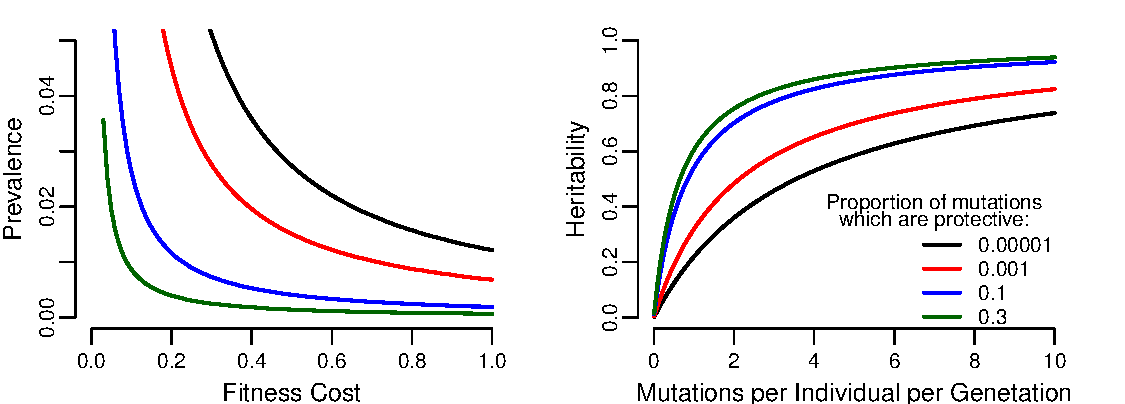
\includegraphics[width=\textwidth]{../figures/SimpleModelSolutions.pdf}
    \caption{Solutions to the model specified by equations \eqref{univariate-bulk-eq} and \eqref{sel-coef}. The left panel shows the diseaes prevalence at equilibrium as a function of the fitness cost for various different choices of the strength of mutation bias. The right panel shows the heritability of disease liability as a function of the total size of the mutational target, again for different strengths of mutational bias.}
    \label{simple-model-solve}
  \end{figure}
  



\subsubsection*{Specific Aim 1: Develop Models Relating Population Genetic Processes with the Architecture of Complex Diseases}

Building on my preliminary studies, I will also model the effects of environmental change, pleiotropy and non-equilibrium demography on the genetic architecture of complex diseases. I will solve these models to obtain closed forms for summaries of genetic architure and disease prevalence. In cases where analytical treatment proves difficult, I will use simulations and other numerical methods to obtain solutions, and all analytical results will be verified in this manner as well. Modeling efforts will be targeted toward identifying how each of these factors affect architecture and prevalence, with the later goal of using GWAS results to ascertain their effects on human diseases (aim 2). With that in mind, a major product of this theoretical aim (not discussed beyond this point) will be a thorough investigation of the identifiability of parameters introduced below, and subsequently a general guidelines to ground future discussions about what aspects of complex genetic disease biology and evolutionary history can or cannot be inferred from GWAS.

\paragraph{Environmental Change}
 
The most straightforward way to model environmental change may also be the most relevant one: namely, to assume that the mean or the variance of the environmental component of liability variance shifts or increases suddenly. We are particularly interested in the scenario where an environmental shift has just occurred (e.g. diet and lifestyle on type 2 diabetes prevalence), but there has not been sufficient time for allele frequencies to evolve away from their previous equilibria. In the case of a shift in the environmental mean, the effect is simply an increase (or decrease) in prevalence such that $P_{new} = 1 - \Phi\left(\Phi^{-1}\left(1-P_{old}\right)-\delta\right)$, where $\delta$ is the shift in the environmental contribution to liability measured in units of the phenotypic standard deviation ($\Phi$, again, is the Gaussian cdf). In the case of a change in the environmental variance, both the prevalence and the heritability are affected. If the environmental variance is increased by an amount $\psi$ (given in units of the pre-change phenotypic variance), then heritability is decreased such that $h^2_{g,new} = \frac{h^2_{g,old}}{1+\psi}$, while prevalence will increase to $P_{new} = 1 - \Phi\left(\frac{\Phi^{-1}\left(1-P_{old}\right)}{1+\psi}\right)$.

Such changes to the environment would affect the architecture observed in GWAS. While the allele frequencies and liability scale effect sizes of mutations would be unchanged, the effect size on the risk scale, estimated in GWAS in terms of the odds-ratio, would be altered. For example, for a mutation with a fixed effect on liability, an environmentally induced increase in prevalence should lead to an increased odds ratio, as a higher prevalence also means that the proportion of individuals whose liability is just shy of the threshold (and who could therefore be pushed over by an extra mutation at a single site) is higher. This suggests that the distribution of odds ratios (e.g. observed in GWAS) together with estimates of the present day prevalence and fitness cost might allow for inference of the size or type of environmental shift, and/or ancestral prevalence. 

In addition to these simple scenarios, I will also study how more involved patterns of environmental change influence disease prevalence and the genetic architecture of risk. For example, we will consider the case where the environmental change occurred sufficiently long ago to have impacted the distribution of allele frequencies, as might plausibly have occurred when archaic humans migrating out of African encountered their new Eurasian environment. 



\paragraph{Pleiotropy}
Mounting vidence suggests that alleles that affect the risk of a given disease often also affects other traits \cite{BulikSullivan:2015jf,Pickrell:2016ko, Visscher:2016fp}, suggesting that the selection acting on such alleles depends not only on their effect on the disease under consideration but also on these pleiotropic effects. I will focus on pleiotropic effects of two kinds. The first are pleiotropic effects on the risk of developing other diseases. An allele which increases the liability for a given disease may also increase or decrease the liability for several other diseases. The selection effect on that allele would therefore by a sum over the effect sizes on difference diseases, weighted according to the fitness cost and prevalence of each disease as in Eq \eqref{sel-coef}. 

I will begin by considering ``isotropic'' models of disease only, in which all diseases have identical parameters (here and below $\Theta_A$ represents collectively all of the parameters of the model, including the number of diseases, their fitness costs and prevalence, mutational bias, etc). Specifically, this assumption ensures that conditional on a mutation's ultimate effects on fitness, the marginal distributions of effects on liability for each disease are identical. Given a specification of parameters, this marginal distribution $(p\left(\alpha \mid s,\Theta_A\right))$ will be derived from geometric considerations of the model. Ultimately, we are interested in an expression for the joint distribution of effect sizes and frequencies (i.e. ``the architecture''). In general, the marginal distributions of effect sizes and frequencies are independent conditional on the selection coefficient, and therefore
\begin{align}
  p\left(\alpha,x \mid \Theta_A\right) = \int p\left(\alpha \mid s,\Theta_A\right) p\left(x \mid s \right) p\left(s\right)\mathrm{d}s
  \label{exp-for-arch}
\end{align}
where the distribution of frequencies, $p\left(x \mid s \right)$, can be computed from diffusion theory \cite{Ewens}, and the distribution of selection coefficients, $p\left(s\right)$, is generally unknown (indeed, its inference is a major goal of aim 2).

The second form of pleiotropy considered will be that due to selection on continuous (i.e. non-disease) traits. I will assume that these traits are subject to stabilizing selection, as decades of work suggest is typical \jb{refs}. Models of stabilizing selection on quantitative traits indicate that at equilibrium, the population is held near the optimum, and selection therefore acts to reduce the contribution to phenotypic variance made by any individual allele. The result is that alleles which impact quantitative traits experience symetric underdominance for fitness (i.e. the minor allele is always selected against), where the strength of selection scales with the square of the effect size on the quantitative trait \cite{Robertson:1956dk}.

Inclusion of pleiotropic effects on quantitative traits will therefore involve specifying the relative proportion of mutational effects on fitness which derive from disease and from continuous traits. The considerations above suggest this problem can be approached by specifying a distribution of dominance coefficients given the homozygous selection coefficient and the parameters of the model (i.e. $p\left(h \mid s , \Theta_A\right)$). Mutations with large effects on disease liability and small effects on continuous traits would exhibit directional selection but with some dominance effect, while those with small effects on diease and large effects on continuous traits would show asymetric underdominance for fitness, as there will generally be selection against the liability increasing allele, but at high frequencies mean fitness might be increased by instead fixing this allele in order to reduce phenotypic variance of the quantitative trait. Specification of this distribution of dominance coefficients in terms of the model parameters will allow a new version of Eq \eqref{exp-for-arch} including a second integral over dominance coefficients, thereby including pleiotropy from both diseases and continuous traits.

Finally, I will eventually relax the ``isometric'' assumption to understand how differences among diseases/traits in their parameters or covariance in mutational effects might alter our understanding.  

% The major objective here is to derive an expression for joint distribution of effect size and allele frequency (i.e. the genetic architecture) as a function of the parameters ($\Theta_A$) which describe the nature of pleiotropy impacting the disease architecture. These two quantities are conditionally independent of one another given the specification of the selection coefficient(s), which suggests a tractable approach for theoretical analysis and for inference (aim 2). The expression for the genetic architecture can be written as an integral over the selection coefficients

% \begin{align}
%   p\left(\alpha,x \mid \Theta_A\right) = \int \int p\left(\alpha \mid s,h,\Theta_A\right) p\left(x \mid s,h \right) p\left(h \mid s , \Theta_A \right)p\left(s\right)\mathrm{d}s \mathrm{d}h.
%   \label{exp-for-arch}
% % \end{align}

% The expression for the distribution of allele frequencies ($p\left(x \mid s,h\right)$) can be computed from standard diffusion theory \cite{Ewens}, and this fact can be leveraged in an inference context (aim 2) to learn the distribution of the selection coeficients ($p\left(s,h\right)$) directly from the data (alternately, plausible distribution can be specified in a theoretical context to understand how differences in the distribution of selection coeffients impact architecture). This leaves specifying the distribution of effect sizes for a given set of selection coefficients and under a given set of parameters governing the effects of pleiotropy ($p\left(\alpha \mid s,h,\Theta_A\right)$) as the primary theoretical task.

% I will approach this problem first by considering simple isotropic models of pleiotropy in which mutations may affect more than one disease/trait, but which lack mutational covariance among diseases or traits. In particulary, I will investigate how the number of pleiotropically related diseases/traits, the strength of selection on them, and the degree of functional overlap among diseases/traits all impact the genetic architecture of disease. I will then consider extensions of the isotropic model in order to understand how covariance among traits affects the dynamics.

I anticipate that the work described here will be useful beyond the specific goals of this proposal. Notably, beyond studying how pleiotropy affects the architecture of one disease, it provides a framework for studying the joint architecture of multiple diseases or quantitative traits together \jb{refs}, and a basis for examining popular models in medical genetics, e.g. that some common diseases are in fact a collections of multiple distinct but biologically related disorders that present similar symptoms\cite{Gottesman:2003ul, Flint:2007ia, Kendler:2010kw, Mitchell:2012hw}. 

% This result of this theoretical work will be a broad framework for studying the effects of pleiotropy which I expect to be applicable beyond the stated aims of this proposal. In addition studying how pleiotropy impacts the architecture of one disease, this work will form a basis for the explicit study of the joint architecture of multiple traits together in a unified framework, and it provies a natural way of examining popular models in medical genetics such as the idea that some common diseases may be in fact be collections of multiple distinct but biologically related disorders which all present similar symptoms. 


\paragraph{Non-Equilibrium Demography}

Recent work has illustrated that the demographic history of a population can have a profound impact on the genetic architecture of complex diseases \cite{Tennessen:2012ek,Keinan:2012kl,Simons:2014fj, Gao:2014dz, Gazave:2013jh, Lohmueller:2014gd}. Specifically, changes in population size, such as the Out of Africa bottleneck and explosive recent growth, affect allele frequencies\cite{Tennessen:2012ek,Keinan:2012kl} by changing the rate of genetic drift and the frequencies at which new mutations enter the population. These effects are modulated by the selection acting on mutations, because more strongly selected mutations tend to be younger and to segregate at lower frequencies\cite{Simons:2014fj}. While the effects of demographic history on genetic variation at a single site under selection are fairly well understood, we lack an understanding of its effects on genetic architecture that is grounded in realistic models of complex diseases.   

To develop such an understanding, I will study how non-equilibrium demography affects genetic architecture under our models of complex disease. Specifically, I will focus on our pleiotropic models and consider three main demographic scenarios: 1) a simple bottleneck, and 2) explosive growth, which will provide qualitative insights about the effects of each, and 3) a demographic model inferred for European populations\cite{Tennessen:2012ek, Schiffels:2014cu}, which will be necessary for inference (aim 2).  Allelic dynamics with selection and non-equilibrium demography are generally not analytically tractable, so my analysis will rely on simulations. Simulating the complete disease models directly may be computationally difficult, as a single simulation would involve running a large population with many loci forward in time. To circumvent this, I will rely on the fact that the dynamics of an individual allele are independent of all other alleles conditional on the global parameters (fitness cost, prevalence, etc), which will allow me to simulate a single allele at a time over a grid of selection parameters and consider the effects on disease risk as a whole as an appropriately weighted grid. My investigation of the preliminary model also suggests that disease prevalence at equilibrium is fairly sensitive to population size. This is significant, specifically because the selection coefficient experienced by a particular allele depends on the disease prevalence. If prevalence evolves over time in response to changes in population size, then selection coefficients will change over time as well, and I will need to incorporate this effect into my simulations as well.

% It is clear from population genetic work over the last decade and a half that demographic events such as the Out of Africa bottleneck and recent explosive population growth have had a significant impact on allele frequencies and therefore potentially on genetic architecture. Recent work from Dr Sella's lab\cite{Simons:2014fj}, and others\cite{Gao:2014dz, Gazave:2013jh, Lohmueller:2014gd} suggests that both the bottleneck and recent growth may have impacted genetic architecture, though the relative importance of each depends on the (as yet unknown) selection coefficients of disease alleles. However, what most work to date on this problem has been done in the context of a single site in a vaccum with a fixed selection coefficient, with no explicit disease phenotype, and therefore no model of the relationship between effect size and selection coefficient.

% I will use simulation based approaches, together with the theory of pleiotropy developed above, to study how the particular course of human demographic history has impacted the evolution of complex disease architecture and prevalence. Population size changes impact architecture through their modulation of the relationship between genetic drift and natural selection. All else being equal, genetic architectures in larger populations will be composed of more rare alleles, due to the increased efficiency of selection, though the precise impact depends on the details of the model. My investigation of the preliminary model also suggests that disease prevalence at equilibrium is fairly sensitive to population size. This is significant, specifically because the selection coefficient experienced by a particular allele depends on the disease prevalence. If prevalence evolves over time in response to changes in population size, then selection coefficients will change over time as well.

\paragraph{Additional Complications}

While the factors listed in this section are obviously not exhaustive, modeling their effects will clearly advance our understanding of the way salient population genetics processes shape the architecture of complex disease. In addition, I will study the sensitivity of my results to variations on the underlying modeling assumptions, e.g. I will analytically assess the impact of large effect mutations which influence liability and use simulations to study the sensitivity of my results to the effects of LD among variants.

% In addition to these major issues, I will study how our results depend on the fidelity of our baseline assumptions. \jb{expand}

% A final theoretical goal will be to obtain an understanding of the extent to which we should expect the various parameters which arise in the investigations described above to be uniquely identifiable, and on the basis of what kinds of data. It seems likely that we will find that there are qualititatively distinct phenomena which lead to similar genetic architecture and disease prevalence. A major product of this theoretical work will therefore be thorough guidelines about what can and cannot be inferred about the population genetics of complex disease from GWAS data, guidelines which we will be able to apply immediately in the development of our inference approaches below. 


\subsection*{Specific Aim 2: Inference of Model Parameters from GWAS of Complex Diseases}

\paragraph{Background}

In principle, we can use results from GWAS in order to test models of genetic architecture and infer their underlying evolutionary parameters. Previous work from the Reich and Altshuler labs has gone the farthest in this direction and is the most closely related to the research proposed in this aim \cite{Agarwala:2013bu, Fuchsberger:2016df, Mancuso:2015cp}.  They employ an Approximate Bayesian Computation approach based on Eyre-Walker’s model of architecture\cite{EyreWalker:2010dn} (see Background and Significance) to infer mutational target sizes and the couplings between effect size and fitness (Eyre-Walker’s $\tau$) that are consistent with GWAS results for type 2 diabetes\cite{Agarwala:2013bu,Fuchsberger:2016df} and prostate cancer\cite{Mancuso:2015cp}. Specifically, they simulate genetic architectures under a grid of possible values for these two parameters, and compare summaries of architecture (e.g., the number of genome-wide significant associations\cite{Agarwala:2013bu} or the proportion of variance explained by SNPs with minor allele frequency < $5\%$\cite{Fuchsberger:2016df,Mancuso:2015cp}) between simulations and GWAS to ascertain the parameter values that are consistent with observations for these diseases. While they are able to rule out the pleiotropic and direct selection extremes ($\tau$ = 0 or 1), they fail to narrow down the range of models much further. Their inferred ranges for target sizes are also unfortunately large. This severely limits the utility of the inferences, e.g., for learning about evolutionary parameters or making predictions about the performance of future mapping strategies.

These pioneering efforts suffer from several notable problems. First, they rely on relatively coarse summary statistics that discard a great deal of information, limiting their ability to constrain the parameter space. Second, they make significant and unjustified assumption, e.g. that the distribution of selection coefficients for GWAS alleles resembles that for substitutions in proteins, despite mulitple lines of evidence that it does not \cite{EyreWalker:2007dl,Pickrell:2014bw,Racimo:2014cb}. Third, as discussed previously (see Background and Significance), the Eyre-Walker model makes some rather \textit{ad hoc} assumptions about the relationship between effect size and selection coefficient, which make biological interpretation of the inferences it produces challenging. I will address each of these concerns in the development of my inference approach.

% I’d end by saying that in moving forward, you will address all of these problems. (no need for a third paragraph)  
% In part this is because the distribution of selection coefficients is usually taken to be gamma (rather than inferred from the data), likely with little real justification. It is also clear that the statistical summaries used for inference by these authors discard a great deal of potentially useful information about the genetic architecture. The Eyre-Walker model is also fundamental not extensible to inference with multiple traits together, which we expect to particularly important in the future as multi-trait GWAS methods continue to mature.\cite{PickrellPairwise,SomeMatthewStephensPaper}

% In each, the authors simulated data under a range of parameter choices for the Eyre-Walker model, and used statistical summaries of the genetic architecture (such as the number of significant variants discovered or the proportion of variance explained by SNPs with minor allele frequency < $5\%$) in an approximate Bayesian computation approach to determine what sort of pleiotropy was most consistent with GWAS data on a partiulcar complex disease.

% \jb{this needs work}
% In general, these studies have been able to exclude extreme models, ruling out scenarios with either perfect coupling (limited/no pleiotropy) or no coupling (i.e. extreme pleiotropy) between a mutation's effect and selection coefficient, as well as providing estimates of the mutational target size. However, the existing approach leaves much to be desired, as further interpretation of inferences based on the Eyre-Walker model in general remains difficult. In part this is because the distribution of selection coefficients is usually taken to be gamma (rather than inferred from the data), likely with little real justification\cite{EyreWalker:2007dl,Racimo:2014cb}. It is also clear that the statistical summaries used for inference by these authors discard a great deal of potentially useful information about the genetic architecture. The Eyre-Walker model is also fundamental not extensible to inference with multiple traits together, which we expect to particularly important in the future as multi-trait GWAS methods continue to mature.\cite{PickrellPairwise,SomeMatthewStephensPaper}

% It is therefore clear that there is a need for an inference approach which A) uses as much of the information available in GWAS data as possible, and B) allows for the estimation of parameters which have biologically meaningful interpretations. 

\paragraph{Approach}
I will develop a general and extensible composite likelihood approach to infer the parameters which govern the evolution of complex genetic disease architecture. Approaching this problem in a likelihood framework will allow for both rigorous model comparisson and parameter estimation\cite{Larribe:2011jb,Coffman:2015by}. The data I will rely on include paired estimates of effect sizes and allele frequencies from loci discovered in GWAS, and eventually, statistical summaries of variance contributed by loci which do not meet genome-wide significance.

The major components of the likelihood include the probability of observing $K$ genome wide significant loci, ($p\left(K \mid \Theta_A , \Theta_S \right)$; which is Poisson conditional on the parameters), the probability density of variants with a given effect size and frequency ($p\left(\alpha_i , x_i \mid \Theta_A \right)$; given by Eq \eqref{exp-for-arch}), and the power to discover such a variant ($H\left(\alpha_i , x_i \mid \Theta_S\right)$, which is already well studied\cite{Sham:2014di}). Here, $\Theta_S$ represents the known parameters of the association study and disease (e.g. the number of cases and controls, disease prevalence), while $\Theta_A$ as above represents the parameters of the model governing the evolution of the disease. The exact parameters denoted by $\Theta_A$ will therefore depend on the specific model being considered, but for example in the case of the isotropic model of pleiotropy from other diseases, would include the mutational target size, distribution of selection coefficients, and number of diseases contributing to pleiotropy.

\begin{wrapfigure}{r}{0.5\textwidth}
  %\captionsetup{width=0.5\textwidth}
    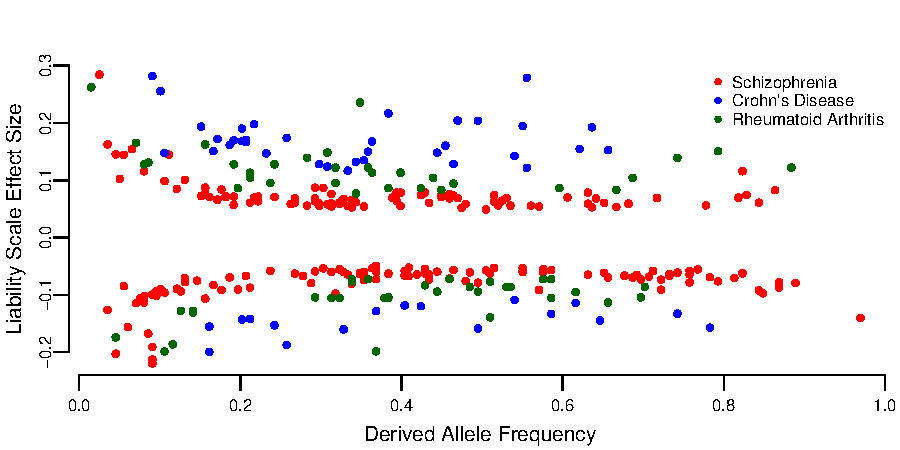
\includegraphics[width=0.5\textwidth]{../figures/JointSpecFig.pdf}
   \caption{The relationship between allele frequency and effect size at known GWAS loci for three different complex diseases. Differences among diseases reflect differences in the underlying parameters which govern their evolution.}
   \label{joint-freq-effect-dist}
 \end{wrapfigure}


% \setlength{\jot}{-17pt}

Intuitively, the number of variants discovered ($K$) in a GWAS of a given sample size places some bounds on the plausible size of the mutational target and on the distribution of effect sizes, and specific knowledge of their effect sizes and frequencies ($\alpha_i$ and $x_i$) provides information about their selection coefficients and the impact of pleiotropy on the genetic architecture (see Fig \ref{joint-freq-effect-dist}). Unfortunately, even in very large GWAS, a significant number of variants will remain undetected, restricting our inference to use only those with the largest effect sizes. We can overcome this limitation by incorporating recently developed methods related to Yang and Visscher's ``GCTA''\cite{Yang:2011hd} that estimate the relationship between minor allele frequency (MAF) and variance explained across all SNPs regardless of whether they are genome wide significant \cite{Speed:2017ec, Evans:2017ce}, as Eq \eqref{exp-for-arch} can be leveraged to make quantitative predictions about this relationship. Intuitively, diseases with genetic architectures dominated by large selection coefficients on individual alleles will have more of the genetic variance explained by rare alleles, though this relationship will be moderated by additional factors such as pleiotropy and demography. Putting this additional factor together with the components discussed above, we can write the likelihood of the model parameters given the data as 
\begin{align*}
  L\left(\Theta_A \mid \{\left(\alpha_i, x_i\right)\}_{i=1}^K , V^*_A, \Theta_S\right) 
  = Pr\left(K \mid \Theta_A , \Theta_S \right) \Bigg( \prod_{i=1}^K Pr\left(\alpha_i , x_i \mid \Theta_A \right) H\left(\alpha_i , x_i \mid \Theta_S\right) \Bigg) p\left(V^*_A\left(x\right) \mid \Theta_A, \Theta_S \right)
\end{align*}
where $p\left(V_A^*\left(x\right) \mid \Theta_A , \Theta_S\right)$ denotes this expression for how variance is distributed among allele frequencies genome-wide. There are at least two clear options for how to approach this part of the inference problem. These include 1) separate alleles into different MAF bins and estimate the proportion of variance explained by alleles in each bin\cite{Lee:2012iu,Evans:2017ce}, or 2) estimating only a single variance component, but weighting the contribution of SNPs with a given frequency to the genetic relationship matrix used for this estimation according to the parameters being inferred ($\Theta_A$).

The ultimate result of this aim will be the first statistical framework for inferring the parameters underlying complex genetic disease architecture and prevalence that is grounded in quantitative and population genetic principles. An open access software package will be made freely available so that other researchers can the inference approaches developed here to their datasets, and so that the method can be improved to incorporate future theoretical advances.

% I will formalize the above intuition into a composite likelihood based inference approach to infer the salient parameters which govern genetic architecture. A general version of this likelihood can be written as

% \begin{multline*}
%   L\left(\Theta_A \mid \{\left(\alpha_i, x_i\right)\}_{i=1}^K , \{V^*_{G,b}\}_{b=1}^B, \Theta_S\right) \\ 
%   = \underbrace{Pr\left(K \mid \Theta_A , \Theta_S \right)}_{\substack{\text{likelihood of observing} \\ \text{K variants under model}}} \Bigg( \prod_{i=1}^K \overbrace{Pr\left(\alpha_i , x_i \mid \Theta_A \right)}^{\substack{\text{likelihood of effect} \\ \text{and frequency under} \\ \text{model (e.g. eq \ref{exp-for-arch})}}} \underbrace{H\left(\alpha_i , x_i \mid \Theta_S\right)}_{\substack{\text{account for power} \\ \text{and false pos rate}}} \Bigg) \prod_b^B \overbrace{Pr\left(V^*_{G,b} \mid \Theta_A, \Theta_S \right)}^{\substack{\text{distribution of variance} \\ \text{from alleles with effects} \\ \text{too small to detect}}}
% \end{multline*}
% The first two terms account for indivivdual genome wide significant variants. The third term upweights and downweights individual alleles in proportion to our confidence that the represent a true association rather than a false positive, and the final term accounts for the proportion of the genetic variance ($V_{G,b}^*$) which can be attributed to alleles in each of $B$ different allele frequency bins, and is not captured by the genome-wide significant variants. Here, $\Theta_A$ represents the parameters to be inferred, which determine the genetic architecture and prevalence, while $\Theta_S$ represents the known parameters of the GWAS, such as the numbers of cases and controls. 

% An advantage of the likelihood approach to inference is that it facilitates model comparison. I will derive expressions for the likelihood under a range of models, and then use model comparison metrics like the widely applicable infromation criteria (WAIC) or leave one out cross validation\cite{Vehtari:2016fm} to determine which model is most consistent with the genetic architecture of the disease. One potential pitfall is that in the case that GWAS variants are in linkage disequilibrium with one another, our approach is a composite rather than full likelihood. Such approaches are commonplace in population genetics, and provide statistically consistent parameter estimates\cite{Wiuf:2006bl}, but they underestimate the uncertainty of those estimates, and can wrongly favor more complex models with more parameters. We can circumvent this obstacle by evaluating model fit and uncertainty via approaches based on the bootstrap. If this proves computationally prohibitive, we may also be able to proceed by adapting approaches from composite likelihood based demographic inference\cite{Coffman:2015by} to our case.  

% An additional advantage of pursuing inference in this likelihood framework is that we will be able to make predictions about the number of variants we should expect to discover, and the distribution of their effect sizes and frequencies, as future GWAS samples sizes are increased. This will allow for continued reassessment of our models of disease into the future, and in cases where multiple qualititatively distinct models fit the available data, we will be able to make forecasts about what sort of sample sizes will be necessary in order to distinguish different models.  


\bibliography{library}
\bibliographystyle{unsrt}
\end{document}
